\markboth{}{}
% Plus petite marge du bas pour la quatrième de couverture
% Shorter bottom margin for the back cover
\newgeometry{inner=30mm,outer=20mm,top=40mm,bottom=20mm}
%insertion de l'image de fond du dos (resume)
%background image for resume (back)
\AddToShipoutPicture*{%
     \put(0,0){%
     \parbox[b][44.2cm]{\paperwidth}{%
          \vfill
          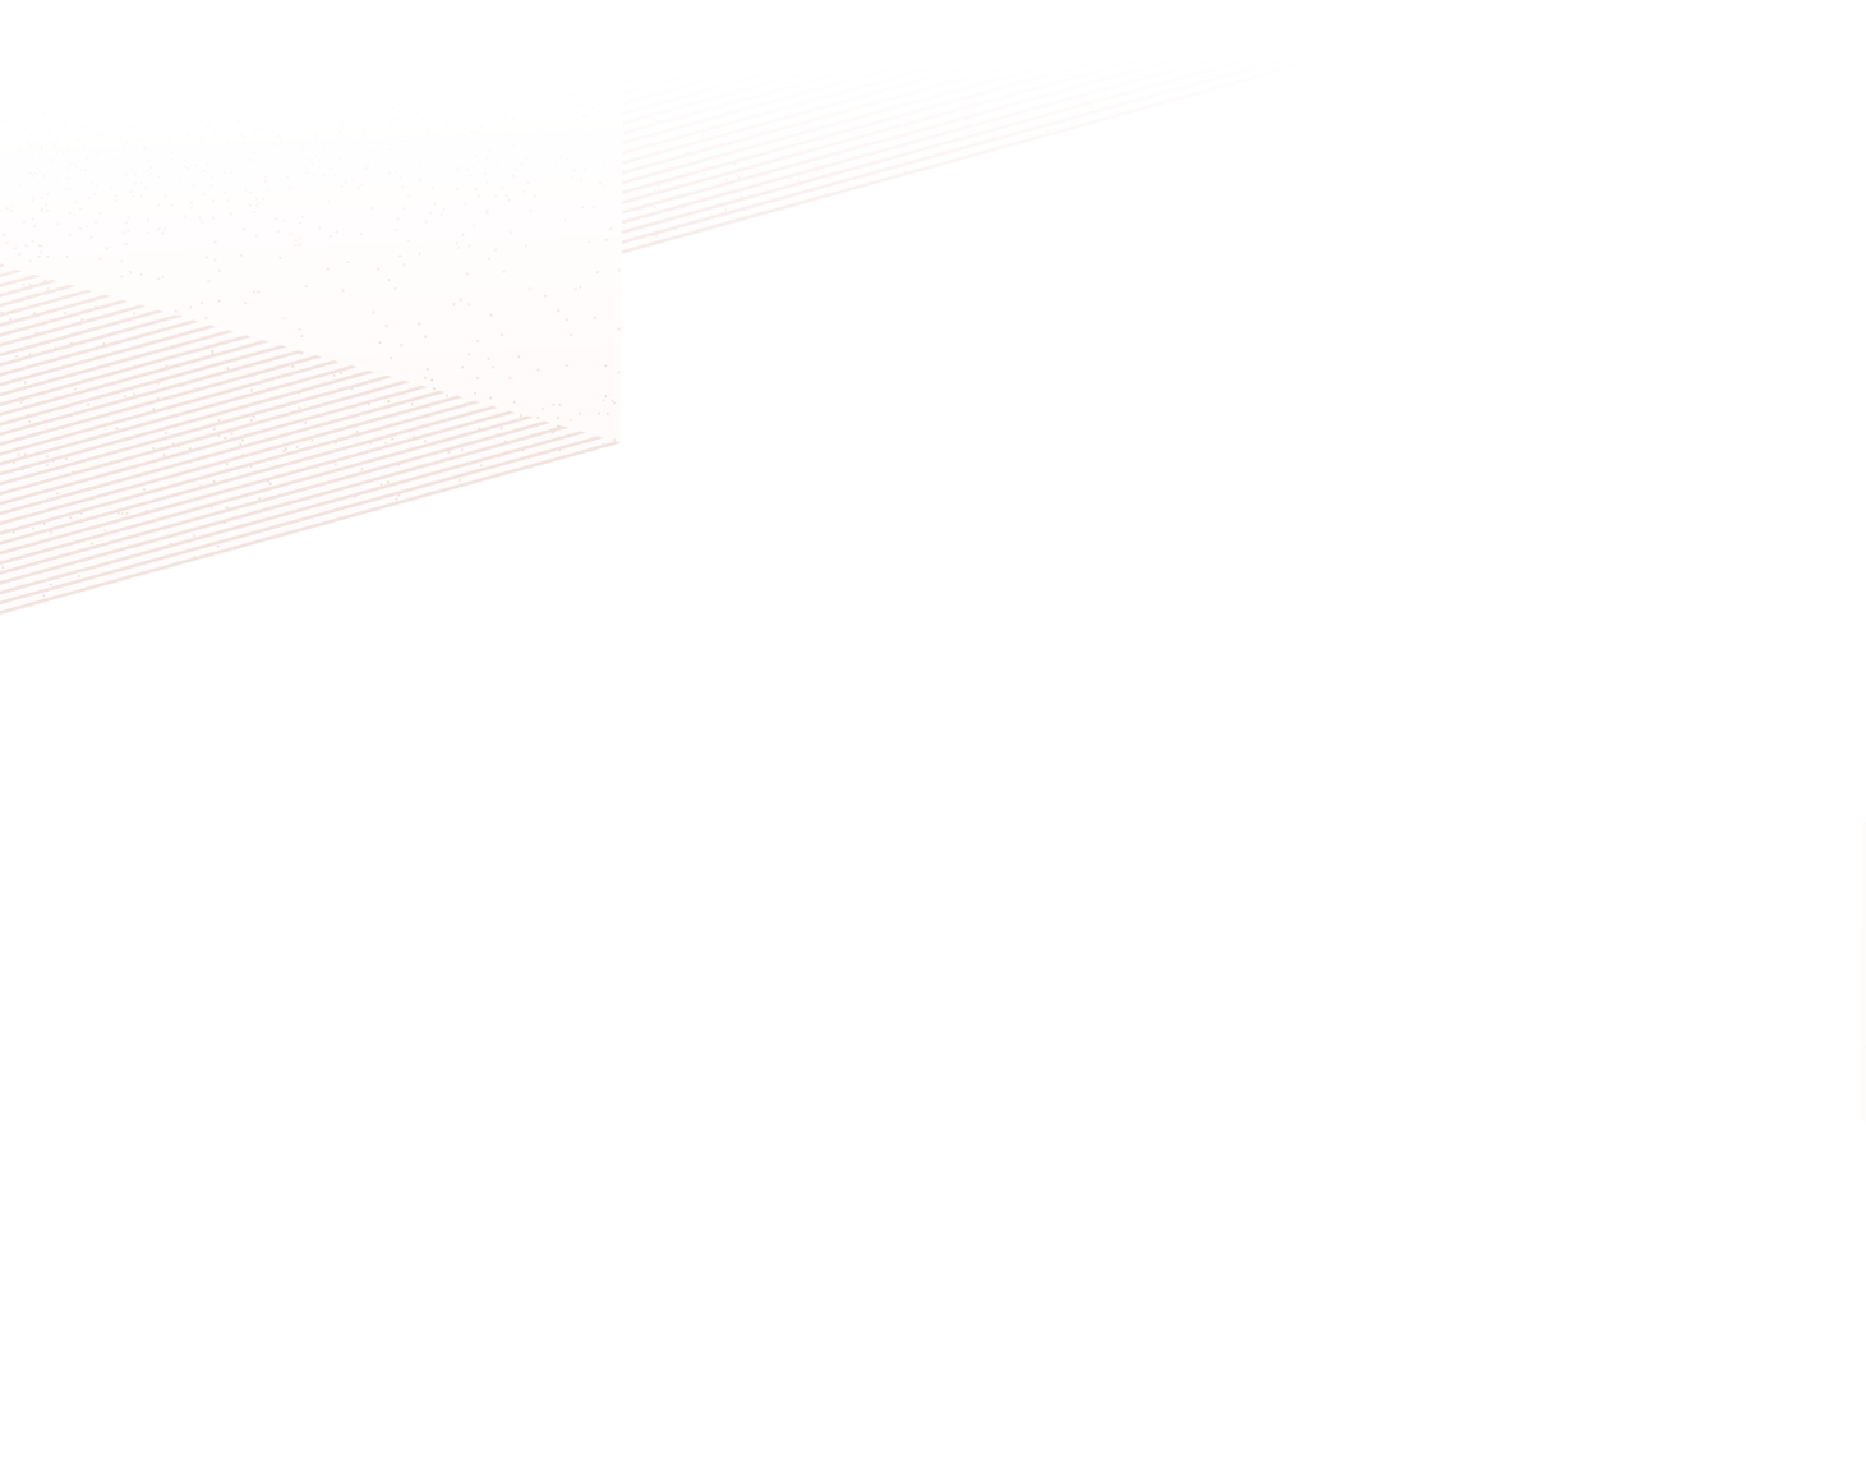
\includegraphics[width=\paperwidth,keepaspectratio]{./Couverture-these/MathSTIC/image-fond-MATHSTIC-dos.png}%
          \vfill
}}}
\pagestyle{empty}
\hspace{1cm}
\begin{tikzpicture}[remember picture,overlay,line width=0mm]
  \draw [draw=white]
    (current page.north west) rectangle (\paperwidth,1);
  \node[xshift=0.03\paperwidth,yshift=2cm,text=white,font=\bf\Large] {
  
\includegraphics[width=5cm]{./Couverture-these/MathSTIC/logo-mathSTIC}
  };
  \hfill
  \node[xshift=.55\paperwidth,yshift=2cm,text=white,font=\bf\Large] {
  
\includegraphics[width=5cm]{./Couverture-these/MathSTIC/logo-etablissements/logoUR1}
  };
\end{tikzpicture}
\par\nobreak
\vspace{1cm}
{\centering \noindent \textcolor{mathSTIC-Color}{\rule{\textwidth}{0.2cm}}}
\vspace{-1cm}
\selectlanguage{french}
\section*{\small\textcolor{mathSTIC-Color}{Titre :} titre (en fran\c cais)..............}
\vspace{-0.2cm}
\noindent{\small\keywordsF{de 3 \`{a} 6 mots clefs}}
\vspace{-0.2cm}
\begin{multicols}{2}
\begin{small}
\begin{spacing}{1}
\noindent \textbf{Resum\'{e} : }Eius populus ab incunabulis primis ad usque pueritiae tempus extremum, quod annis circumcluditur fere trecentis, circummurana pertulit bella, deinde aetatem ingressus adultam post multiplices bellorum aerumnas Alpes transcendit et fretum, in iuvenem erectus et virum ex omni plaga quam orbis ambit inmensus, reportavit laureas et triumphos, iamque vergens in senium et nomine solo aliquotiens vincens ad tranquilliora vitae discessit.
Hoc inmaturo interitu ipse quoque sui pertaesus excessit e vita aetatis nono anno atque vicensimo cum quadriennio imperasset. natus apud Tuscos in Massa Veternensi, patre Constantio Constantini fratre imperatoris, matreque Galla.
Thalassius vero ea tempestate praefectus praetorio praesens ipse quoque adrogantis ingenii, considerans incitationem eius ad multorum augeri discrimina, non maturitate vel consiliis mitigabat, ut aliquotiens celsae potestates iras principum molliverunt, sed adversando iurgandoque cum parum congrueret, eum ad rabiem potius evibrabat, Augustum actus eius exaggerando creberrime
docens, idque, incertum qua mente, ne lateret adfectans. quibus mox Caesar acrius efferatus, velut contumaciae quoddam vexillum altius erigens, sine respectu salutis alienae vel suae ad vertenda opposita instar rapidi fluminis irrevocabili impetu ferebatur.
Hae duae provinciae bello quondam piratico catervis mixtae praedonum.
\end{spacing}
\end{small}
\end{multicols}



\vspace{0.5cm}
{\centering \noindent \textcolor{mathSTIC-Color}{\rule{\textwidth}{0.2cm}}}
\vspace{-1cm}
\selectlanguage{english}
\section*{\small\textcolor{mathSTIC-Color}{Title:} title (en anglais)..............}
\vspace{-0.2cm}
\noindent{\small\keywordsE{de 3 \`{a} 6 mots clefs}}
\vspace{-0.2cm}
\begin{multicols}{2}
\begin{small}
\begin{spacing}{1}
\noindent \textbf{Abstract: }Eius populus ab incunabulis primis ad usque pueritiae tempus extremum, quod annis circumcluditur fere trecentis, circummurana pertulit bella, deinde aetatem ingressus adultam post multiplices bellorum aerumnas Alpes transcendit et fretum, in iuvenem erectus et virum ex omni plaga quam orbis ambit inmensus, reportavit laureas et triumphos, iamque vergens in senium et nomine solo aliquotiens vincens ad tranquilliora vitae discessit.
Hoc inmaturo interitu ipse quoque sui pertaesus excessit e vita aetatis nono anno atque vicensimo cum quadriennio imperasset. natus apud Tuscos in Massa Veternensi, patre Constantio Constantini fratre imperatoris, matreque Galla.
Thalassius vero ea tempestate praefectus praetorio praesens ipse quoque adrogantis ingenii, considerans incitationem eius ad multorum augeri discrimina, non maturitate vel consiliis mitigabat, ut aliquotiens celsae potestates iras principum molliverunt, sed adversando iurgandoque cum parum congrueret, eum ad rabiem potius evibrabat, Augustum actus eius exaggerando creberrime
docens, idque, incertum qua mente, ne lateret adfectans. quibus mox Caesar acrius efferatus, velut contumaciae quoddam vexillum altius erigens, sine respectu salutis alienae vel suae ad vertenda opposita instar rapidi fluminis irrevocabili impetu ferebatur.
Hae duae provinciae bello quondam piratico catervis mixtae praedonum.
\end{spacing}
\end{small}
\end{multicols}

% Rétablit les marges d'origines
% Restore original margin settings
\restoregeometry
